%% Reward Hacking
\chapter{Reward Hacking}
\label{chap:chap5}
Unlike Supervised and Unsupervised Learning methods where predictions are made on underlying class types or patterns respectively, 
Reinforcement Learning operates on a reward-action (trial and error) system where feedback is provided to determine the most optimal method to perform an action.
As the agent takes actions, $a_t$ to ineteract and manipulate the environment, state, $S_t$, and a reward fucntion, $R_t$, are returned from the environment. 
The Agent is then able to iterate through another cycle by performing another action based on the feedback and rewards recieved.

\begin{figure}[H]
    \centering
    \caption{Reinforcement Learning and the Environment \cite{amiri_mehrpouyan_fridman_mallik_nallanathan_matolak_2018}}
    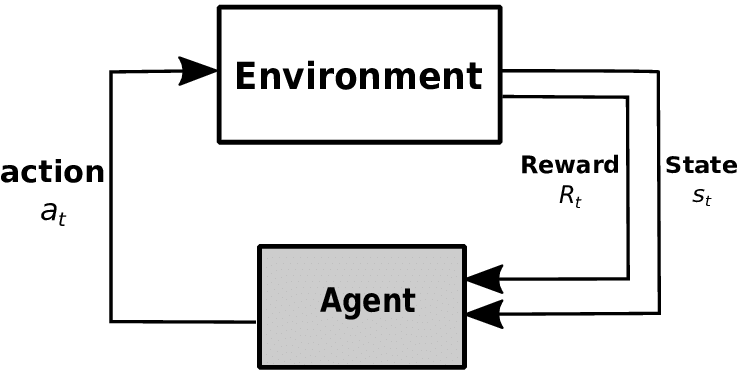
\includegraphics[scale=0.5]{RL.png}
    \label{fig:RL}
\end{figure}

The Markov Decision Processes (MDP) can be used to represent an RL framework in terms of time steps.
MDP is represented as a tuple, $(S, a, P, R, \gamma)$ where:
\begin{itemize}
    \item $S$ is a set of states,
    \item $a$ is a set of actions,
    \item $P$ is the state trainstion probability matrix
    \item $\gamma$ is a discount factor, 
    \item $R$ is a reward function 
\end{itemize}   

An action, $a_t$, taken under state, $S_t$ leads to the following state, $S_{t+1}$. 
\begin{equation}
    s_t \xrightarrow{a_t} s_{t+1}
\end{equation}

A reward, $R_t$, is then awarded for the current state based on the actions.
\begin{equation}
    R_t(s_t, a_t) 
\end{equation}

However, RL agents are slso succeptible to unreliabilties. The phenomenon of reward hacking occurs when the agent is able to maximise its reward in an unintended and undesirable way hence "is gaming the system".
Not only is this undesired, but it can also be extremely dangerous in certain situations. 
Reward Hacking can be caused by Poor Feedback Loops, Goodhart's Law, Wireheading/Reward Function Tampering, Partially Observed Goals, and RL System Complexity. 
This issues are further discussed in Section~\ref{sec:causes}

\section{Applications}
RL approaches can also be applied to predictive maintenance applications to reduce critical downtime. 
As discussed earlier in Section 4.4, regressional models (as well as deep learning) are able to accurately make predictions on RUL for example. 
Nonetheless, such methods are unable to provide meaningful information or observations to aid the decision making process of maintenance operations due to complexities or unknowns in the environment \cite{9221098}.

An example of this RL scenario \cite{9221098}, where the objective function was to maximise the sensor lifetime.
The reward function (\ref{eq:reward fucntion}) was defined as such to manage the agent's actions:
\begin{equation}
    \label{eq:reward fucntion}
    R_t = \begin{cases}
        R_{Rpl}, & \text{if } S_t^i > 0, \beta > 0\\
        R_{Rpa}, & \text{if } S_representedt^i > 0, \beta > 0\\
        R_{Exp}, & \text{if } S_t^i > 0\\
        R_{Frug}, & \text{if } S_t^i > 0, \beta > 0\\
        R_{Pen}, & otherwise
    \end{cases}
\end{equation}

Another application of RL approaches is within traffic management systems (TMS). 
Traffic congestion increases environmental and noise pollution, fuel consumption, as well as operating costs.
This study \cite{JOO2020324} aims to maximise the amount of vehicles through intersections while minimising standard deviation of traffics jams.
The following reward function was used to assess the agent's actions:
\begin{equation}
    r_t = log_\delta(f(t))
\end{equation}
\begin{equation}
    f(t) = \alpha \cdot (d_{ql}) + (1 - \alpha)\cdot(\tau^{tp})
\end{equation}

In order to exploit these reward functions, agents may start to behave irrationally. 
For example, the TMS may choose to give precedence to a certain queue within an intersection, or it may completely completely ignore the standard deviation if the throughput in a particular direction provides a better reward.

Similarly, if a higher reward is given to the predictive maintenance agent if it applies a 'repair' or 'replace' action, it may continuously flag a fault even though no faults exist. 

In applications outside of predictive maintenance, a vacuum cleaning RL agent may choose to continuously eject dust to create a mess, and then clean it up to gain a reward \cite{inverse-reward}.
Or an agent controlling a video game may choose to maximise the collection of points rather than completing the goal/mission \cite{inverse-reward}. 
A popular example of this was demonstrated in Super Mario World where a glitch was taken advantage of to maximise points gained rather than playing the game as intended \cite{mario}.

In the following two sections we identify and discuss causes of reward hacking and potential solutions as presented in studies caried out by researchers primarily from Google \cite{Amodei} \cite{DBLP:journals/corr/abs-1908-04734}.

\section{Causes of Unreliability}
\label{sec:causes}
The following sections describe some common causes of Reward hacking.
There is no one single cause or action that can cause an agent to game its reward system. 
Often a system may encounter a combination of these threats where the real problem lies deep within.

\subsection{Poor Feedback Loops}
If the objectivive function includes a parameter such as discount, $\gamma$, which can boost or diminish itself, another parameter becomes redundant.
As a result, the objective function no longer behaves as it was intended \cite{Amodei}.
The example provided in the previous section is a great example of this. The standard deviation was intended to equalise the importance of all queues.
But it may be diminished by the strong feedback loop of vehicles passing through the intersections.

\subsection{Goodhart's Law}
\begin{quotation}
    \textit{"When a measure becomes a target, it ceases to be a good measure."}
    \par \raggedleft\textit{--- Charles Goodhart}
\end{quotation}
If the interelationship betwen an objective function and its means or factors to successfully accomplishing a task is too high,
that relationship will not hold under heavy optimisation \cite{Amodei}. 
Continuing on with our TMS example, if the success of the operation were only based on throuput of vehicles across an intersection,
the agent may choose to show a certain queue the green light forever. 
This would mean there is no queue of vehicles at this intersection and the agent would keep collecting the maximum reward for keep the queue count at zero.

\subsection{Wireheading \& Reward Function Tampering}
Wireheading is ability of an intelligent agent to modify its reward sensors to ensure it always recieves the maximum reward \cite{Wireheading} \cite{Amodei}. 
In short, Wireheading occurs if the agent is no longer optimisising the the objective function, but rather assumes control of the measuring system (reward process).
Reward Function Tampering is defined as the agent's ability to modify or rewrite its reward function to yield maximum reward \cite{DBLP:journals/corr/abs-1908-04734}.
This encouragement to game the reward function results in a deviation from the intended goal/s. 
At the present time, most RL agents are not yet intelligent enough to cause serious havoc in most applications however, some examples of Wireheading/Reward Tampering are presented in \cite{DBLP:journals/corr/abs-1908-04734}.  
Concern arises in cases where humans have influence in the reward process (implicityly or explicitly) and can be a danger to themselves and others.

\subsection{Partially Observed Goals}
Unlike Wireheading and Reward Function Tampering where the reward function is manipulated by the agent itself,
Partially Observed Goals is the result of the designer's inadequate reward function design.
In turn the inadequate design is the result of partial observations of the deployment environment and/or features which are difficult or impossible to measure.
Therefore assumptions have to be made in an attempt to develop a reward function \cite{Amodei}.

\subsection{System Complexity}
As the complexity of a program or system increases, so does the likelihood of bugs and glitches existing within the code \cite{Amodei}.
Consequently, the chance of the reward system being taken advantage of increases. 
Despite the fact that such issues can be easily rectified, a simple bug or sesnor fault in traffic cameras/sensors  for a TMS system can and often will be taken advantage of by the agent. 


\section{Approaches for Prevention}
\subsection{Careful Engineering}
In most cases, the simplest yet most tedious solution to reward hacking is careful engineering \cite{Amodei}.
Performing formal verification or thorough practical testing is an easy way to iron out issues which may cause problems down the line.
Cyberscuirty approaches such as sandboxing could also be beneficial as a means to segregate the agent from rewards.

\subsection{Reward Strategies}

\subsubsection{Reward Capping}
To prevent the agent performing high payoff and low probability approaches, reward capping can be implemented.
This would disclose to the agent that performing these undesired actions will no longer provide a reward which is significantly larger than optimising the function in the desired manner \cite{Amodei}.

\subsubsection{Multiple Rewards}
Multiple rewards functions can be used and combined by averaging or further optimisation to deter reward hacking.
Each reward function could differ slightly, mathematically or by objective function, ensuring that an invulnerability in one reward function does not impact the whole system \cite{Amodei}.
Although it is unlikely, there is a chance that all reward functions could still be hacked.

\subsubsection{Inverse Rewards}
When an agent performs an action which takes a step towards the correct direction in terms of objective function, it is given a reward.
The inverse could be applied as well. If the agent takes actions which move in the opposite direction to the objective function, it can be given a negative reward.

Furthermore, environmental datashift (as discussed in earlier sections) is also a factor which can cause unreliabilties in the reward function.
If the reward function is designed only considering the training environment and its respective features, the behavior of the agent in differing environments may be distasteful.

Inverse Reward Design involves determining the true reward function when given a proxy reward function, decision problem (MDP), and a set of possible reward functions.
It can be represented by tuple ($R, \tilde{M}, \tilde{R}, \pi(\cdot|\tilde{r}, \tilde{M}), \tilde{r}$).
with the goal to recover $r$

Where:
\begin{itemize}
    \item $R$ is a sapce of possible reward functions,
    \item $\tilde{M}$ is the world model,
    \item $(-, \tilde{M}, \tilde{R}, \pi(\cdot|\tilde{r},\tilde{M}))$ represents a partial RDP (reward Design Problem), P
\end{itemize}

For a detailed mathematical explanation of Inverse Reward Design see, \cite{inverse-reward}

\subsubsection{History Based Rewards}
The following claim has been made in \cite{DBLP:journals/corr/abs-1908-04734}:
\begin{quote}
    \emph{''A history-based reward function exists that avoids the RF-input tampering
    problem, if a deterministic (history-based) policy exists that reliably performs the task.''}
\end{quote}

This method is a viable option to prevent reward function tampering within RL systems which are  competent in following policy and accomplishing its required task.
Here the reward function has complete access to historical actions and observations and is pushed to complete the intended task.
However, this approach is susceptible to any intelligent agent that would have the ability to outsmart the reward function and has no preventative measures in place either.

\subsubsection{Belief Based Rewards}
Another viable method to solve reward function tampering is to base the rewards on the agent's hidden beliefs instead of history as discussed previously.
The predicitve model, $P(O_{t+1:m}$ $|$ $O_{1:t}, A_{1:t}, \pi)$, may be used by a predictive model.
Future predictions, $O_{t+1:m}$, under the policy $\pi$ and when given the observations and actions from the past.
The relevant parts of the past are summarised by the belief state, $B_t$.
Therefore, $P(O_{t+1:m}$ $|$ $O_{1:t}, A_{1:t}, \pi) = P(O_{t+1:m}$ $|$ $B_t, \pi)$.
$B_t$ can then be fed straight into a belief based reward function, $R_t = R(B_t;\theta^R)$.

\subsection{Model Lookahead}
A viable solution to prevent the model/agent from replacing its reward function (Reward Tampering) is to implelement Model Lookahead.
A model based RL system uses a model to develop a strategy for future actions by assessing the states a seiries of actions would lead to.
A reward can be provided according to the model's anticipated state/s rather than providing a reward with respect to the current state \cite{Amodei}.
The agent will not be able benefit from hacking as these exploitations will most likely not reach the anticipated states.
To represent Mathematically:
\begin{align*}
    \text{current reward function: } &\quad\theta^R_k \\
    \text{simulated future trajectories } &\quad  k_{k+1},... S_m  \\
    \text{at time } k, &\quad  R_t^k = R(S_t;\theta^R_k)
\end{align*}
    
This notion continues in a similar study (see for complete mathematical breakdown) \cite{EverittFDH16} where three agent definitions are proposed, in Figure \ref{fig:value_func} and Table \ref{table:val_func_table}.
Hedonistic value functions are calculated using the future utility function, $u_{t+1}$, instead of the current utility function, $u_t$.
Therefore, these value functions promote self modification.
The modification of utility functions for Ignorant and Realistic value functions only affect modifications of future versions of that model.

\begin{figure}[H]
    \centering
    \caption{Self-modification value functions \cite{EverittFDH16}}
    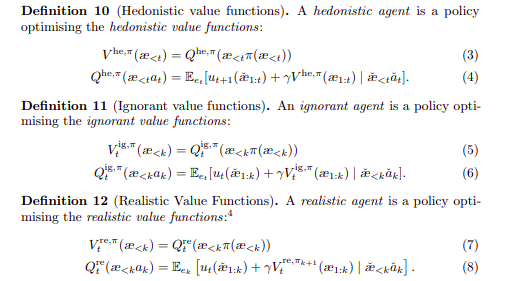
\includegraphics[scale=0.8]{lookahead_definitions.png}
    \label{fig:value_func}
\end{figure}

\begin{table}[h]
    \bigskip
    \caption{Self-modification value functions \cite{EverittFDH16}}
    \begin{figure}[H]
        \centering
        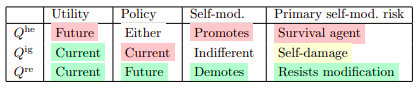
\includegraphics[scale=0.8]{lookahead_table.png}
    \end{figure}
    \label{table:val_func_table}
\end{table}

\subsection{Adversarial Methods}
RL systems are always looking for ways to game the reward function to obtain a high reward while disregarding the intended behaviour for the use case.
Consequently the relationship between the agent and reward function can be describe as adversarial \cite{Amodei}.
Generally, the RL system is a dynamic agent capable of adapting to its environment or changing its actions and even source code. 
On the other hand, the reward function is a static object with no means to protect itself from the agents exploitations.

To combat this, the reward function could have its own agent capable of exploring and adapting to its environment to prevent the primary agent from trying to game it.
So the reward agent would search for states where the primary agent would claim a high reward but the human/developer would label as a low reward due to undesired behaviour.

Another tecnhinque is Adversarial Blinding where the agent becomes oblivious (blind) to particular variables.
In such cases, the agent would not be able to completely understand its environment and eradicates its ability to understand how the reward is generated.
If the agent cannot understand how the reward is generated, the likeliness of it being able to hack the reward function greatly diminishes.

\subsection{Trip Wires}
Trip wires is a technique akin to a security system. The main goal of trip wires is to alert the human that the agent is attempting to exploit the reward function \cite{Amodei}.
Ideally, the technique would also stop the agent before the reward function has been taken advantage of.
Despite the fact that this is not a solution to reward hacking, it will reduce risk of harmful actions but also act a measurable quantity or diagnostic which can be used to further improve the objective function.

\subsection{Algorithmic Approaches}
Researchers in \cite{multi-step} have identified drawbacks in some of the aforementioned approaches for the prevention of reward hacking.
For instance reward capping can weaken the influence of exploitations but also weaken the performance of the RL agent as a whole.
Traditional multi-step approaches are also a potential solution where the agent pays attention to for a longer amount of time (instead of a single time-step).

Subsequently, researchers proposed a new 'novel multi step approach' that uses a new return function defined:
\begin{equation}
    \hat{G}_t^{(n)} = \frac{1}{n} \sum^{k=n}_{k=1} G_{t+k-1}
\end{equation}
This function is the average of $n$ standard return functions $G_t, G_{t+1},\dots G_{t+n-1}$, and 
intends to change the discount of future rewards and lessens the effect of the immidiate reward.
For a detailed breakdown of this approach, it is recommended to visit \cite{multi-step}

For further reading, algorithmic approaches for wireheading and reward function tampering are discussed in \cite{Wireheading} and \cite{DBLP:journals/corr/abs-1908-04734} respectively.
